\subsubsection{Q10.20 data 09202021 10082021 grouped by scenario \& group}

\begin{comment}
                        EFPR        EO      EFNR     n    pvalue
(frauth, majority)  0.447368  0.552632  0.500000  19.0  0.661128
(frauth, minority)  0.566667  0.433333  0.500000  15.0  0.414216
(icu, majority)     0.470588  0.529412  0.500000  17.0  0.980270
(icu, minority)     0.545455  0.454545  0.772727  11.0  0.745603
(rent, majority)    0.452381  0.547619  0.261905  21.0  0.858984
(rent, minority)    0.583333  0.416667  0.583333  12.0  0.598642
\end{comment}

\begin{table}[h]
    \centering
    \begin{tabular}{|c|c|c|c|c|c|c|}
        \hline
        scenario & group & EFPR & EO & EFNR & n & p-value\\
        \hline
        frauth & majority & 0.447 & \textbf{0.553} & 0.500 & 19.0 & 0.661\\
		frauth & minority & \textbf{0.567} & 0.433 & 0.500 & 15.0 & 0.414\\
		icu & majority & 0.471 & \textbf{0.529} & 0.500 & 17.0 & 0.980\\
		icu & minority & \textbf{0.545} & 0.455 & \textbf{0.773} & 11.0 & 0.746\\
		rent & majority & 0.452 & \textbf{0.548} & 0.262 & 21.0 & 0.859\\
		rent & minority & \textbf{0.583} & 0.417 & \textbf{0.583} & 12.0 & 0.599\\
		
        \hline
    \end{tabular}
    \caption{Grouped by scenario group}
    \label{tab:my_label}
\end{table}
\begin{figure}[h]
    \centering
    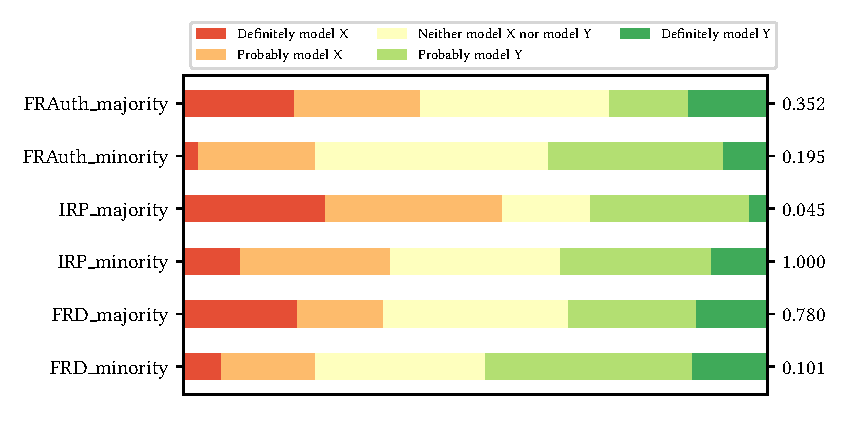
\includegraphics[width=0.8\textwidth]{figures/Q10.20/09202021_10082021/Q10.20_scenario_group.pdf}
    \caption{Grouped by scenario \& group}
    \label{fig:my_label}
\end{figure}
